\documentclass[oneside,14pt]{extarticle}
\usepackage[utf8]{inputenc}
\usepackage[english,ukrainian]{babel}
\usepackage{amssymb,amsfonts,amsmath,amsthm,mathtext,textcomp}

\usepackage[includehead, headsep=0pt, footskip=0pt, top=2cm, bottom=2cm, left=2cm, right=1cm]{geometry}
\usepackage{indentfirst}
\usepackage[onehalfspacing]{setspace}
\usepackage[headings]{fancyhdr}
\usepackage{etoolbox}
\usepackage{flafter}
\usepackage{listings}
\usepackage{graphicx}
\usepackage{float}
\usepackage[labelsep=period]{caption}
\lstset{
	breaklines=false
}
\usepackage{array}
\fancyhf{}
\renewcommand{\headrulewidth}{0pt}
\pagestyle{fancy}
\fancyfoot[R]{\thepage}
\lstset{breaklines=true,}
\graphicspath{ {./pictures} }

\lstset{
	language=c,
	tabsize=4,
	keepspaces,
	showstringspaces=false,
}
\graphicspath{ {./pictures} }
\setlength{\parindent}{4em}
\setlength\tabcolsep{5px}

\newcommand\subject{Моделювання та аналіз програмного забезпечення}
\newcommand\lecturer{доцент кафедри ПЗ \\ Сердюк П.В.}
\newcommand\teacher{викладач кафедри ПЗ \\ Микуляк А.В.}
\newcommand\mygroup{ПЗ-22}
\newcommand\lab{3}
\newcommand\theme{Твірні шаблони проектування}
\newcommand\purpose{Здобути навички використання твірних шаблонів проектування при моделюванні програмних систем}

\begin{document}
\begin{normalsize}
	\begin{titlepage}
		\thispagestyle{empty}
		\begin{center}
			\textbf{МІНІСТЕРСТВО ОСВІТИ І НАУКИ УКРАЇНИ\\
				НАЦІОНАЛЬНИЙ УНІВЕРСИТЕТ "ЛЬВІВСЬКА ПОЛІТЕХНІКА"}
		\end{center}
		\begin{flushright}
			\textbf{ІКНІ}\\
			Кафедра \textbf{ПЗ}
		\end{flushright}
		\vspace{70pt}
		\begin{center}
			\textbf{ЗВІТ}\\
			\vspace{10pt}
			до лабораторної роботи № \lab\\
			\textbf{на тему}: “\textit{\theme}”\\
			\textbf{з дисципліни}: “\subject”
		\end{center}
		\vspace{50pt}
		\begin{flushright}
			
			\textbf{Лектор}:\\
			\lecturer\\
			\vspace{10pt}
			\textbf{Виконав}:\\
			
			студент групи \mygroup\\
			Коваленко Д.М.\\
			\vspace{10pt}
			\textbf{Прийняв}:\\
			
			\teacher\\
			
			\vspace{28pt}
			«\rule{1cm}{0.15mm}» \rule{1.5cm}{0.15mm} 2023 р.\\
			$\sum$ = \rule{1cm}{0.15mm}……………\\
			
		\end{flushright}
		\vspace{\fill}
		\begin{center}
			\textbf{Львів — 2023}
		\end{center}
	\end{titlepage}
		
	\begin{description}
		\item[Тема.] \theme.
		\item[Мета.] \purpose.
	\end{description}

	\section*{Завдання}
Розробити твірні шаблони проектування відповідно до прецедентів обраного варіанту
ігрової логіки. Вибрати один з прецедентів, для якого найбільш доцільно застосувати твірний
шаблон (не всі прецеденти цього потребуватимуть).

	Представити діаграму класів ігрового проекту (із відображенням на ній використаних
	шаблонів).

	\section*{Хід виконання}
	
	\begin{figure}[H]
		\centering
		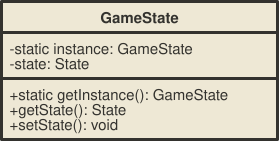
\includegraphics[scale=1]{singleton}
		\caption{UML діаграма реалізації шаблону Singleton}
	\end{figure}
	
	\begin{small}
		\begin{lstlisting}
export class GameMenu extends Node {
	private static instance: GameMenu;
	public startGame: () => void = () => {
		console.error("startGame method is not implemented");
	};
	private isInitial: boolean = true;
	private isOpened: boolean = true;
	
	private constructor() {
		super("div", "game-menu-icon", "<span>Menu</span>");
		this.bootstrap();
	}
	
	private bootstrap(): void {
		if (this.isInitial) {
			this.openMenu();
		}
		this.getNode().addEventListener("click", () => {
			if (!this.isOpened && !this.isInitial) {
				this.openMenu();
			}
		});
	}
	
	public static getInstance(): GameMenu {
		if (!GameMenu.instance) {
			GameMenu.instance = new GameMenu();
		}
		
		return GameMenu.instance;
	}
}
		\end{lstlisting}
	\end{small}
	
	\begin{figure}[H]
		\centering
		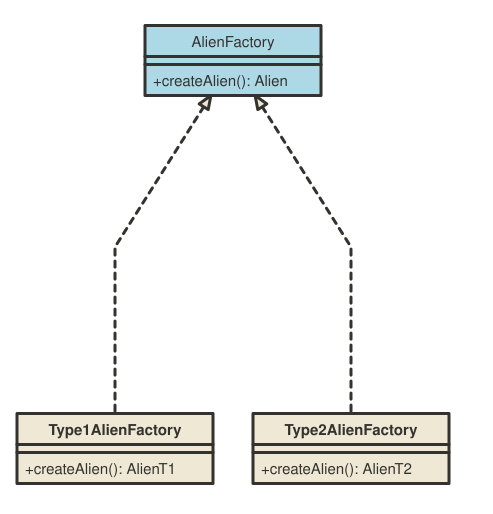
\includegraphics[width=\textwidth]{abstract-factory}
		\caption{UML діаграма реалізації шаблону Abstract Factory}
	\end{figure}
	
	\begin{small}
		\begin{lstlisting}
interface CardDeck {
	createAttackCardDeck(): Card[];
	createHealCardDeck(): Card[];
	createDefenseCardDeck(): Card[];
}

class AttackCardSet implements CardDeck {
	private numberOfHealCards: number = 5;
	private numberOfAttackCards: number = 7;
	private numberOfDefenseCards: number = 3;
	
	createAttackCardDeck(): Card[] {
		let cards = [];
		for (let index = 0; index < this.numberOfAttackCards; index++) {
			cards.push(CardFactory.createCard("attack"));
		}
		return cards;
	}
	createHealCardDeck(): Card[] {
		let cards = [];
		for (let index = 0; index < this.numberOfHealCards; index++) {
			cards.push(CardFactory.createCard("attack"));
		}
		return cards;
	}
	createDefenseCardDeck(): Card[] {
		let cards = [];
		for (let index = 0; index < this.numberOfDefenseCards; index++) {
			cards.push(CardFactory.createCard("attack"));
		}
		return cards;
	}
}

class DefenseCardSet implements CardDeck {
	private numberOfHealCards: number = 3;
	private numberOfAttackCards: number = 5;
	private numberOfDefenseCards: number = 7;
	
	createAttackCardDeck(): Card[] {
		let cards = [];
		for (let index = 0; index < this.numberOfAttackCards; index++) {
			cards.push(CardFactory.createCard("attack"));
		}
		return cards;
	}
	createHealCardDeck(): Card[] {
		let cards = [];
		for (let index = 0; index < this.numberOfHealCards; index++) {
			cards.push(CardFactory.createCard("attack"));
		}
		return cards;
	}
	createDefenseCardDeck(): Card[] {
		let cards = [];
		for (let index = 0; index < this.numberOfDefenseCards; index++) {
			cards.push(CardFactory.createCard("attack"));
		}
		return cards;
	}
}

class HealCardSet implements CardDeck {
	private numberOfHealCards: number = 7;
	private numberOfAttackCards: number = 5;
	private numberOfDefenseCards: number = 3;
	
	createAttackCardDeck(): Card[] {
		let cards = [];
		for (let index = 0; index < this.numberOfAttackCards; index++) {
			cards.push(CardFactory.createCard("attack"));
		}
		return cards;
	}
	createHealCardDeck(): Card[] {
		let cards = [];
		for (let index = 0; index < this.numberOfHealCards; index++) {
			cards.push(CardFactory.createCard("attack"));
		}
		return cards;
	}
	createDefenseCardDeck(): Card[] {
		let cards = [];
		for (let index = 0; index < this.numberOfDefenseCards; index++) {
			cards.push(CardFactory.createCard("attack"));
		}
		return cards;
	}
}

export function createDeck(type: string): Card[] {
	const deck = [];
	if (type === "attack") {
		const factory = new AttackCardSet();
		deck.push(...factory.createAttackCardDeck());
		deck.push(...factory.createHealCardDeck());
		deck.push(...factory.createDefenseCardDeck());
	} else if (type === "defense") {
		const factory = new DefenseCardSet();
		deck.push(...factory.createDefenseCardDeck());
		deck.push(...factory.createHealCardDeck());
		deck.push(...factory.createAttackCardDeck());
	} else if (type === "heal") {
		const factory = new HealCardSet();
		deck.push(...factory.createHealCardDeck());
		deck.push(...factory.createAttackCardDeck());
		deck.push(...factory.createDefenseCardDeck());
	}
	return deck;
}
		\end{lstlisting}
	\end{small}
	
	\begin{figure}[H]
		\centering
		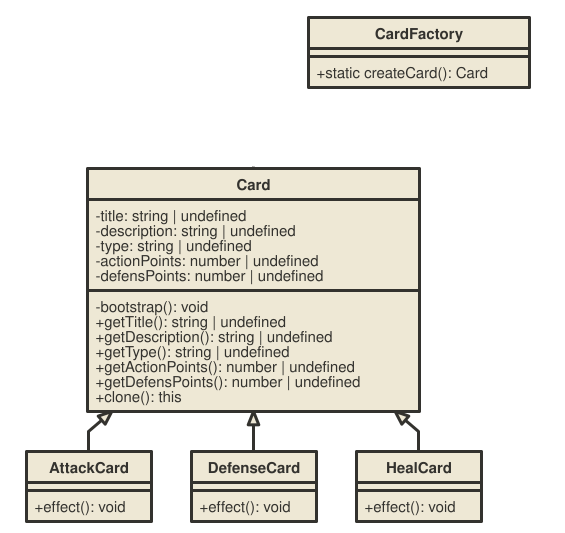
\includegraphics[width=\textwidth]{factory}
		\caption{UML діаграма реалізації шаблону Factory}
	\end{figure}
	
	\begin{small}
		\begin{lstlisting}
class AttackCard extends Card {
	effect(): void {
		console.log("Dealing damage");
	}
}

class DefenseCard extends Card {
	effect(): void {
		console.log("Defending");
	}
}

class HealCard extends Card {
	effect(): void {
		console.log("Healing");
	}
}

export class CardFactory {
	static createCard(type: string): Card {
		if (type === "attack") {
			return new AttackCard();
		} else if (type === "heal") {
			return new HealCard();
		} else if (type === "defense") {
			return new DefenseCard();
		}
		throw new Error("Unknown card type");
	}
}
		\end{lstlisting}
	\end{small}
	
	\begin{figure}[H]
		\centering
		\includegraphics[width=\textwidth]{builder}
		\caption{UML діаграма реалізації шаблону Builder}
	\end{figure}
	
	\begin{small}
		\begin{lstlisting}
interface CardBuilder {
	setTitle(title: string): void;
	setDescription(description: string): void;
	setType(type: string): void;
	setActionPoints(value: number): void;
	setDefensePoints(value: number): void;
}

class AttackCardBuilder implements CardBuilder {
	private card: Card;
	
	private bootstrap(): void {
		fetch('cards.json')
		.then(response => response.json())
		.then(data => {
			const cardData = data[Math.floor(Math.random() * data.length)];
			this.setTitle(cardData.title);
			this.setDescription(cardData.description);
			this.setType(cardData.type);
			this.setTitle(cardData.title);
			this.setActionPoints(cardData.actionPoints);
			this.setDefensePoints(cardData.defensPoints);
			this.appendChild(this.createTitle());
			this.appendChild(this.createDescription());
			this.appendChild(this.createType());
		});
	}
	
	constructor() {
		this.card = new Card();
	}
	
	setTitle(title: string): void {
		this.card.title = title;
	}
	
	setDescription(description: string): void {
		this.card.description = description;
	}
	
	setType(type: string): void {
		this.card.type = type;
	}
	
	setActionPoints(value: number): void {
		this.card.actionPoints = value;
	}
	
	setDefensePoints(value: number): void {
		this.card.defensPoints = value;
	}
}

		\end{lstlisting}
	\end{small}
	
	\begin{figure}[H]
		\centering
		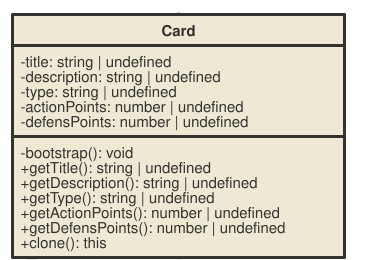
\includegraphics{prototype}
		\caption{UML діаграма реалізації шаблону Prototype}
	\end{figure}
	
	\begin{small}
		\begin{lstlisting}
export class Card extends Node {
	private title: string | undefined;
	private description: string | undefined;
	private type: string | undefined;
	private actionPoints: number | undefined;
	private defensPoints: number | undefined;
	
	constructor() {
		super("div", "card");
		this.bootstrap();
	}
	
	private bootstrap(): void {
		// this.appendChild(this.createTitle());
		// this.appendChild(this.createDescription());
		// this.appendChild(this.createType());
	}
	
	public getTitle(): string | undefined {
		return this.title;
	}
	
	public getDescription(): string | undefined {
		return this.description;
	}
	
	public getType(): string | undefined {
		return this.type;
	}
	
	public getActionPoints(): number | undefined {
		return this.actionPoints;
	}
	
	public getDefensPoints(): number | undefined {
		return this.defensPoints;
	}
	
	public clone(): this {
		const clone = Object.create(this);
		return clone;
	}
}

		\end{lstlisting}
	\end{small}
	
	\section*{Висновки}
	   Під час виконання лабораторної роботи я здобув навички використання твірних шаблонів проектування при моделюванні програмних систем.
\end{normalsize}
\end{document}
